\documentclass[12pt, a4paper]{article}
\usepackage{xeCJK} %中文字體
\usepackage{hyperref} %引用url連結
\usepackage{listings} %引用程式碼
\usepackage{graphicx} %引用圖片
\usepackage{fontawesome5} %引用icon
\lstset{language=Python}
\lstset{basicstyle=\footnotesize}
%\lstset{frame=lines}
%\lstset{caption={2LayerNeuralNetwork.py set input}}
%\lstset{label={lst:code_direct}}
\graphicspath{{./summary/}}
\setCJKmainfont{SimSun} %設定中文字體
\usepackage[]{caption2}
\renewcommand{\figurename}{圖.} %設定圖片標示名稱
\usepackage[margin=1.5cm]{geometry} %設定頁面邊緣

\title{Neural Network in Python Summary}
\author{Kuo Lung Chien\\簡國龍}

\begin{document}
\maketitle

\textbf{\href{https://www.notion.so/codes-40723150-80bd6b7f30e4423f950a04f4447a70ab}{\underline{2LayerNeuralNetwork.py}}}
\begin{itemize}
\item 定義input(X)和output(Y)\\
\begin{lstlisting}
X = np.array(([0,0,0],[0,0,1],[0,1,0], \
  [0,1,1],[1,0,0],[1,0,1],[1,1,0],[1,1,1]), dtype=float)\\
y = np.array(([1], [0], [0], [0], [0], \
  [0], [0], [1]), dtype=float)
\end{lstlisting}
\end{itemize}

\begin{itemize}
\item 設定神經元及權重\\
\begin{lstlisting}
def __init__(self):
    # X1,X2,X3(自訂義input的神經元數量)
    self.inputLayerSize = 3
    # Y1(自訂義output的神經元數量)   
    self.outputLayerSize = 1
    # Size of the hidden layer(自訂義hiddenLayer的神經元數量)          
    self.hiddenLayerSize = 4 
        
    # 設定第一層權重為隨機數值,input--->hidden
    self.W1 = \
    np.random.randn(self.inputLayerSize, self.hiddenLayerSize)
        
    # 設定第二層權重為隨機數值,hidden--->output
    self.W2 = \
    np.random.randn(self.hiddenLayerSize, self.outputLayerSize)
\end{lstlisting}
\end{itemize}

\begin{itemize}
\item feedForward(前饋)\\
\begin{lstlisting}
def feedForward(self, X):
    """
    第一層的動態方程式(activation function)輸入(z)
    z(activation function)= 
    第一層所有神經元的input*weights總和輸入到
    第二層的其中一個神經元
    """
    self.z = np.dot(X, self.W1)
	
    """
    第一層的動態方程式(activation function)輸出(a)
    z2(a) = 動態方程式(activation function)用Sigmoid function算法
    """
    self.z2 = self.activationSigmoid(self.z)

    """
    第二層的動態方程式(activation function)輸入(z)
    z3(activation function) = 
    第二層所有神經元的input*weights總和輸入到
    輸出層的(其中一個)神經元
    """
    self.z3 = np.dot(self.z2, self.W2)
	
    """
    第二層的動態方程式(activation function)輸出(a)
    o(a) = 動態方程式(activation function)用Sigmoid function算法
    """
    o = self.activationSigmoid(self.z3)

    # 回傳出前饋結果
    return o
\end{lstlisting}

\end{itemize}
\begin{itemize}
\item backwardPropagate(反向傳播)\\
\begin{lstlisting}
def backwardPropagate(self, X, y, o):
    # 計算輸出誤差
    self.o_error = y - o

    # 利用Sigmoid function微分一次來修正輸出誤差(錯誤、error)
    self.o_delta = self.o_error*self.activationSigmoidPrime(o)

    # 隱藏層的輸出誤差*權重
    self.z2_error = self.o_delta.dot(self.W2.T)

    # 將Sigmoid function算法用在隱藏層輸出誤差(錯誤、error)
    self.z2_delta = 
    self.z2_error*self.activationSigmoidPrime(self.z2)

    # 修正第一層權重數值,input--->hidden
    self.W1 += X.T.dot(self.z2_delta)
    # 修正第二層權重數值,hidden--->output
    self.W2 += self.z2.T.dot(self.o_delta)
\end{lstlisting}
\end{itemize}

\begin{itemize}
\item trainNetwork(訓練流程)\\
\begin{lstlisting}
def trainNetwork(self, X, y):
    # 前饋循環 
    o = self.feedForward(X)
    # 反向傳播值
    self.backwardPropagate(X, y, o)
\end{lstlisting}
\end{itemize}

\begin{itemize}
\item activationSigmoid\\
\begin{lstlisting}
def activationSigmoid(self, s):
    # activation function
    # 使用Sigmoid function算法(S-curve)
    return 1/(1+np.exp(-s))
\end{lstlisting}
Sigmoid function 
$$\sigma(x)=\frac{1}{1-e^{-x}}$$\\
\end{itemize}

\begin{itemize}
\item activationSigmoidPrime(sigmoid function一次微分)\\
\begin{lstlisting}
def activationSigmoidPrime(self, s):
    return s * (1 - s)
\end{lstlisting}
\href{https://towardsdatascience.com/derivative-of-the-sigmoid-function-536880cf918e}{\underline{First derivative of Sigmoid function}}
$$\sigma(x)'=\sigma(x)[1-\sigma(x)]$$
\end{itemize}

\begin{itemize}
\item saveSumSquaredLossList(儲存損失函數值)\\
\begin{lstlisting}
def saveSumSquaredLossList(self,i,error):
    lossFile.write(str(i)+","+str(error.tolist())+'\n')
\end{lstlisting}
\end{itemize}

\begin{itemize}
\item saveWeights(儲存權重值)\\
\begin{lstlisting}
def saveWeights(self):
    np.savetxt("weightsLayer1.txt", self.W1, fmt="%s")  #第一層權重
    np.savetxt("weightsLayer2.txt", self.W2, fmt="%s")  #第二層權重
\end{lstlisting}
\end{itemize}

\begin{itemize}
\item predictOutput(結果輸出)\\
\begin{lstlisting}
def predictOutput(self):
    print("Predicted XOR output data based on trained weights: ")
    print("Expected (X1-X3): \n" + str(xPredicted))
    print("Output (Y1): \n" + str(self.feedForward(xPredicted)))
\end{lstlisting}
\end{itemize}

\begin{itemize}
\item Epochs(疊代次數,feedForward+backprogation運算完算一次疊代)\\
\begin{lstlisting}
# 訓練疊代次數
trainingEpochs = 1000
\end{lstlisting}
\end{itemize}

\begin{figure}[hbt!]
\center
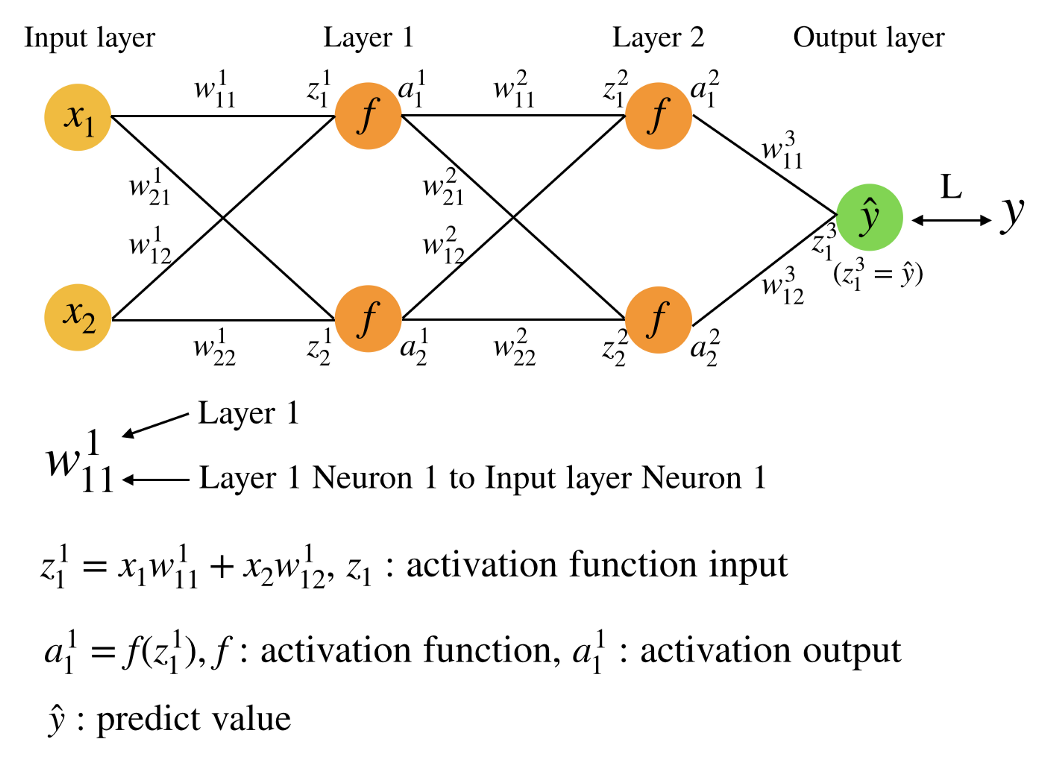
\includegraphics[height=7cm]{nn_network}
\label{fig:Nerual network}
\caption{Nerual network}
\end{figure}
\newpage
\textbf{\href{https://www.notion.so/codes-40723150-80bd6b7f30e4423f950a04f4447a70ab}{\underline{TensorFlowKeras.py}}}

\begin{itemize}
\item 定義input(X)和output(Y)\\
\begin{lstlisting}
X = np.array(([0,0,0],[0,0,1],[0,1,0],\
    [0,1,1],[1,0,0],[1,0,1],[1,1,0],[1,1,1]), dtype=float)
# X是三輸入XOR邏輯閘

y = np.array(([1], [0], [0], [0], [0],\
    [0], [0], [1]), dtype=float)
# Y是輸出神經網路
\end{lstlisting}
\end{itemize}

\begin{itemize}
\item 神經網絡設定\\
\begin{lstlisting}
model = tf.keras.Sequential() 
#sequential定義modle為層狀結構

model.add(Dense(4, input_dim=3, activation='relu', use_bias=True))
'''
add是從最上層開始加入,Dense是密集連線的神經網路,
4:輸出空間(神經元,輸出到4個神經元),input_dim:輸入神經元個數,
activation:定義啟動函數使用的類型,use_bias:使用偏差,True開啟。
從inputlayer輸出到hiddenlayer的設定
'''

#model.add(Dense(4, activation='relu', use_bias=True))
model.add(Dense(1, activation='sigmoid', use_bias=True))
# 從hiddenlayer輸出到outputlayer的設定

model.compile(loss='mean_squared_error', optimizer='adam',\
              metrics=['binary_accuracy'])
'''
配置訓練模組,loss funsion:用maen squared error(差平方誤差),
optimizer:優化器,用adam function,
metrics:計算準確率,用binary_accuracy
'''

print (model.get_weights())#印出回傳的正確權重

history = model.fit(X, y, epochs=2000, validation_data = (X, y))
'''
訓練模型給予固定epochs,迭代收集到的資料,
validation_data:評估準確率(不包含在訓練裡面)
'''
\end{lstlisting}
\end{itemize}
\href{https://www.tensorflow.org/api_docs/python/tf/keras/layers/ReLU}{\underline{ReLU}}
\begin{itemize}
\item $max\_value$:輸出後最大值上限
\item $negative\_slope$:負斜率係數
\item $threshold$:可通過的數值界線
\end{itemize}
$$f(x)=max(0,x)$$
\newpage
Mean squared error(MSE)
\begin{figure}[hbt!]
\center
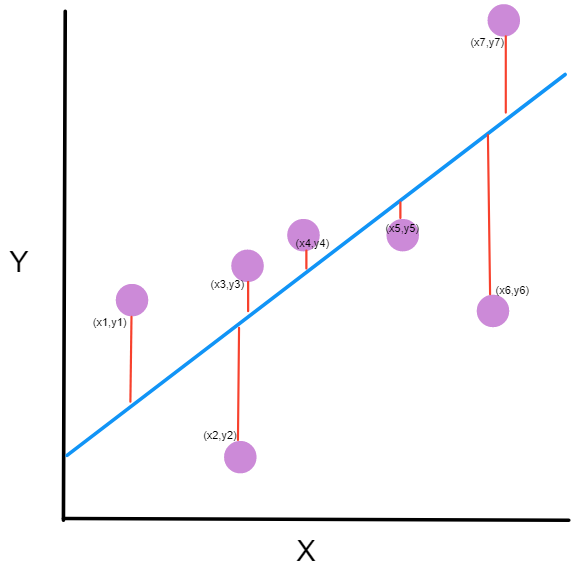
\includegraphics[width=8cm]{MSE}
\caption{Mean Squared Error}
\end{figure}
$$MSE=\frac{1}{n}\sum^{n} _{i=1}(y_i-\overline{y}_i )^2$$\\
\begin{itemize}
\item 紀錄\\
\begin{lstlisting}
model.summary()
# 摘要資料使用在分析和可視化,為了確認訓練架構在符合預期方向

loss_history = history.history["loss"] 
#回傳紀錄事件(loss)到history物件,取得fit方法的模組回傳值
numpy_loss_history = np.array(loss_history) 
#將loss_history數值存成array
np.savetxt("loss_history.txt", numpy_loss_history, delimiter="\n")
#將numpy_loss_history存成loss_history.txt,並將每筆資料用換行符號隔開

binary_accuracy_history = history.history["binary_accuracy"]
#回傳紀錄事件(binary_accuracy)到history物件
numpy_binary_accuracy = np.array(binary_accuracy_history) 
#將binary_accuracy_history數值存成array
np.savetxt("binary_accuracy.txt", numpy_binary_accuracy, delimiter="\n")
#將numpy_binary_accuracy存成binary_accuracy.txt,並將每筆資料用換行符號隔開
\end{lstlisting}
\end{itemize}
\begin{itemize}
\item 結果
\begin{lstlisting}
print(np.mean(history.history["binary_accuracy"])) 
#印出平均binary_accuracy記錄到的數值
result = model.predict(X ).round() 
#替輸入樣本產生輸出預測
print (result) 
#印出結果
\end{lstlisting}
\end{itemize}
\end{document}